\documentclass[12pt,dvipsnames,svgnames,x11names]{article}
\usepackage{../mit}

\allowdisplaybreaks
%
\thispagestyle{empty}%
\pagestyle{plain}%
%
\begin{document}%
\pagecolor{gray!50}
\begin{center}
  \begin{center}
  \vspace*{\fill}
  \textsc{\LARGE Dynamic Programming}
  \par\bigskip
  \textsc{By:}
  \par\bigskip
  \textsc{\LARGE Dustin Smith}
  \vspace*{\fill}
\end{center}
\end{center}

\newpage
Let's discuss dynamic programming. What is dynamic programming? The content of this right up
comes from \href{https://www.youtube.com/watch?v=oBt53YbR9Kk}{Dynamic Programming--Learn to Solve Algorithmic Problems \& Coding Challenges}
\begin{definition}
	Dynamic Programming is both a mathematical optimization method and computer programming 
	method.
\end{definition}
\noindent
With dynamic programming, we can take two approaches memoization and tabulation. We will start with
examining brute force methods and how to apply memoization. First, consider the Fibonacci series.
Let's refresh. The Fibonacci numbers are \(0, 1, 1, 2, 3, 5, 8, \ldots\).  We can define the Fibonacci 
numbers as 
\begin{align*}
	F_n & = F_{n - 2} + F_{n - 1}\\
	F_0 & = 0\\
	F_1 & = 1
\end{align*}
Let's look at the classic recursion method for the Fibonacci series.
\begin{python}
def fin(n: int) -> int:
  if n < 2:
    return 1
  return fib(n - 2) + fib(n - 1)
\end{python}
What would be the steps for \(fib(7)\)?
\begin{figure}[h]
	\centering
	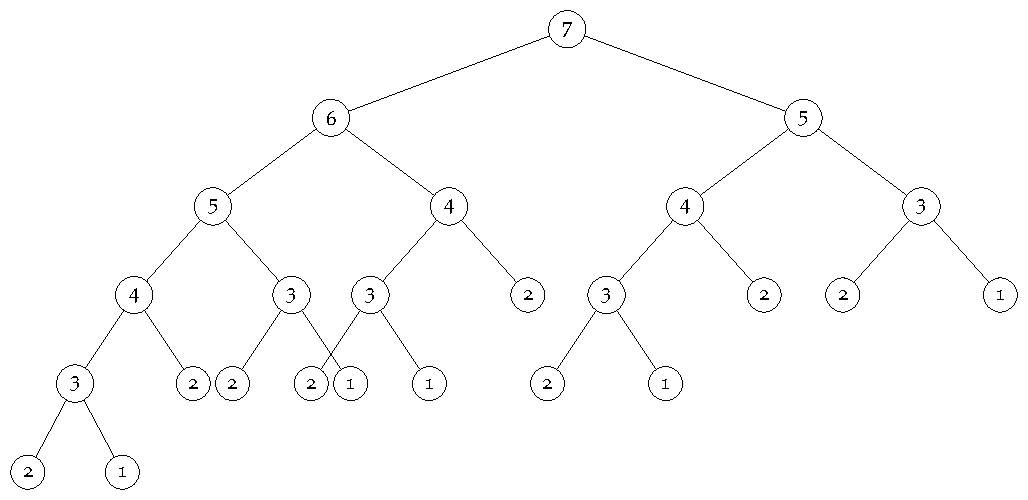
\includegraphics[width=6in]{dp_fib.pdf}
	\caption{Steps for the binary tree of \(fib(7)\).}
	\label{fig:fib_binary_tree}
\end{figure}
What would be the time complexity of the brute force algorithm? We can see that each node has two 
children and the height of the tree is \(n = 7\). That is, we have \(2^n\) steps with brute force so
\(\theta(2^n)\), exponential time complexity. We can generalize the brute force binary steps to be
\(\theta(m^n)\) where \(n\) is the height of tree and \(m\) is the number of elements per child. What 
would be the space the complexity? Whenever we get to a leaf, we reach the end of the stack. In order
to get the next leaf, we must pop stack. Therefore, we use \(n\) stack calls which is the height of the tree,
\(\theta(n)\), linear space complexity. From \cref{fig:fib_binary_tree}, we see we have overlapping sub
problems, namely \(fib(5)\), \(fib(4)\), and \(fib(3)\). This is dynamic programming when we can 
decompose a problem into smaller instances of the same sub problems.
\par\medskip
Let's implement our Fibonacci function but now with memoization.
\begin{python}
def fib_memo(n: int, memo: Dict[int, int]=None) -> int:
  if memo is None:
    memo = {}
  if n in memo:
    return memo[n]
  if n < 2:
    return 1
    
  memo[n] = fib_memo(n - 2, memo) + fib_memo(n - 1, memo)
  return memo[n]
\end{python}
How does our binary tree change in the case of memoization?
\begin{figure}[h]
	\centering
	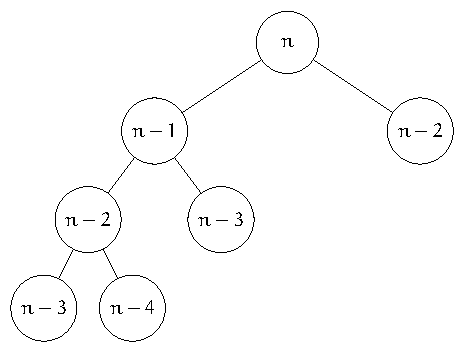
\includegraphics[width=3in]{fib_memo.pdf}
	\caption{Steps for the binary tree of \(fib(n)\) memoization.}
	\label{fig:fib_memo}
\end{figure}
We now have roughly \(2\cdot n\) nodes. That is, our time complexity is now linear of \(\theta(n)\) with
space complexity of \(\theta(n)\) for the dictionary. We were able to go from exponential to linear.
\par\medskip
Let's no look at a traveler on a 2D grid. We begin in the top-left corner and end in the bottom-right
corner. We can only move down or to the right. In how many ways, can we travel to the goal on a 
grid with dimensions \(m\times n\)? First, we will consider some base cases. If either \(m\) or \(n\) are 
zero, then we don't have a grid so we would have zero ways. What if our grid was \(1\times 1\)? There
is only one way since the start is the finish. We can represent our grid traveler problem as tree where
each node is the coordinate pair of position and root of the tree would be the size of the grid.
\begin{figure}[h]
	\centering
	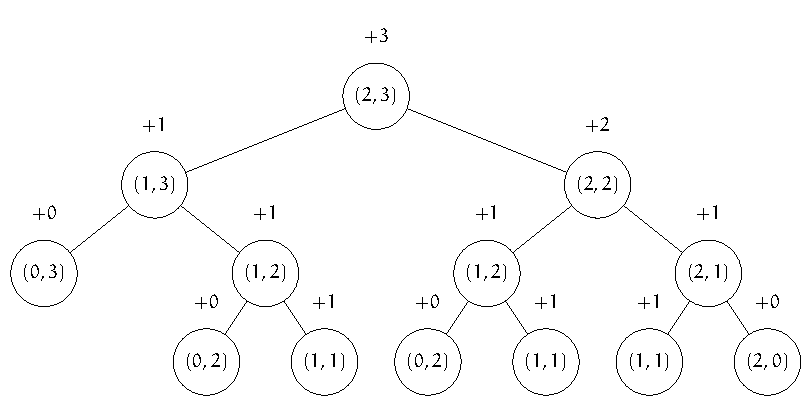
\includegraphics[width=4in]{grid_traveler.pdf}
	\caption{Binary tree for our grid traveler problem of a \(2\times 3\) grid.}
	\label{fig:grid_travel}
\end{figure}
The leaf nodes \cref{fig:grid_travel} are related to our base cases of \(0\) for a grid with with a zero 
column or row and \(1\) for a \(1\times 1\) square grid. Starting from the leafs, we can label the number
of ways with either \(+0\) or \(+1\) for each node. The parent nodes will be the sum of the number of 
ways of the children up to the root.  I have left of the leafs that already have a \(0\) for an \(m\) or \(n\).
However, we can see the height of the tree would be \(m + n\). Each node will have at most two children
so \(\theta (2^{m + n})\).
\begin{python}
def grid_traveler(m: int, n: int) -> int:
  if m == 1 and n == 1:
    return 1
  if m == 0 or n == 0:
    return 0
    
  return grid_traveler(m - 1, n) + grid_traveler(m, n - 1)
\end{python}
For space complexity, the stack would at most have \(m + n\) calls so \(\theta(n + m)\) is our complexity.
\par\medskip
Now, let's implement the grid traveling problem using memoization.
\begin{python}
def grid_traveler_memo(m: int, n: int, memo: Dict[str, int]=None) -> int:
  if memo is None:
    memo = {}
  
  key = f"{m}, {n}"
  if key in memo:
    return memo[key]
    
  if m == 1 and n == 1:
    return 1
  if m == 0 or n == 0:
    return 0
    
  memo[key] = grid_traveler_memo(m - 1, n, memo) + \ 
    grid_traveler_memo(m, n - 1, memo)
  return memo[key]
\end{python}
What would our time and space complexities be? We would have \(m\cdot n\) combinations now as
opposed to \(2^{m + n}\) steps. Thus, our new time complexity \(\theta (m\cdot n)\). Our space
complexity would still be \(\theta (m + n)\). We have been able to improve greatly from exponential
time complexity.
\par\medskip
Now that we have seen a few examples of turning a recursive brute force algorithm into a the 
dynamic programming variant of memoization, we should discuss some guidelines for using 
memoization.
\begin{enumerate}
	\item Determine a recursive solution.
	\item Make it efficient.
\end{enumerate}
What does this mean? We need to visualize it as a tree, implement the tree using recursion where the
leaves are our base cases, and test it. Once we do this, we can move onto adding a memo, add the
base cases to return memo values, and store return values in the memo.
\par\medskip

\end{document}




